\documentclass[../../main.tex]{subfiles}

\begin{document}
\newcommand{\drawcells}[3]{%
    \begin{tikzpicture}
        \foreach \j in {1,...,#1} {
            % Draw each cell
            \node[draw, fill=#3!20, minimum width = \linewidth/#1, minimum height=0.5cm, align=center] (cell\j) at (\j*\linewidth/#1, 0) {#2};
        }
    \end{tikzpicture}}
\section{Guided Vectorization and Data Types for Vector Intrinsics}
\subsection{Vectorization Clauses}
\begin{description}
    \item[aligned] ~\\ This clause tells the compiler that every element of an array $a$ is $n$-byte aligned if one uses \texttt{\#pragma opm simd aligned(a, n)}. The compiler employs this information to effectively vectorize the code section.
    \bigskip
    \item[safelen] ~\\ Imagine we had the following code:
    \begin{lstlisting}
a[0] = b[0];
for (int i = 1; i < n; i++) {
    a[i] = a[i-1] * (i % 2) + b[i];
}
    \end{lstlisting}
    We have a data dependency, but only every second iteration: iteration $i$, where $i$ is odd, depends on $i-1$. Iteration $i$ and $i+1$ are completely independent, however. Hence, we can vectorize the loop with a vector length of $2$. To specify this, we use the \texttt{safelen} clause like so:
    \begin{lstlisting}
a[0] = b[0];
#pragma omp simd safelen(2)
for (int i = 1; i < n; i++) {
    a[i] = a[i-1] * (i % 2) + b[i];
}
    \end{lstlisting}   
    \bigskip
    \item[reduction] ~\\ This clause has the same functionality when paired with \texttt{simd} as when paired with \texttt{paraller for}: It will reduce a variable by an associative operation. But instead of reducing it over multiple threads, we use vectorization for reducing. I imagine that the reduced variable itself will be vectorized, so that the in loop we can employ vector operations, and at the end the elements in the resulting vector will get reduced.
\end{description}

\newpage
\subsubsection{AVX512 data types}
\begin{figure}[h]
\resizebox{\textwidth}{!}{ % Scale to the width of the text
\begin{tabular}{ r c l }
    \texttt{\_\_m512} & \drawcells{16}{F}{blue} & \texttt{16x 32-bit float} \\
    \texttt{\_\_m512d} & \drawcells{8}{D}{green} & \texttt{8x 64-bit double} \\
    \texttt{\_\_m512i} & \drawcells{47}{}{red} & \texttt{64x 8-bit byte} \\
    \texttt{\_\_m512i} & \drawcells{32}{s}{red} & \texttt{32x 16-bit short} \\
    \texttt{\_\_m512i} & \drawcells{16}{i}{red} & \texttt{16x 32-bit integer} \\
    \texttt{\_\_m512i} & \drawcells{8}{ll}{red} & \texttt{8x 64-bit long} \\
    \texttt{\_\_m512i} & \drawcells{4}{dqw}{red} & \texttt{4x 128-bit quad} \\
    \texttt{\_\_m512i} & \drawcells{2}{qqw}{red} & \texttt{2x 256-bit integer} \\
    \texttt{\_\_m512i} & \drawcells{1}{dqqw}{red} & \texttt{1x 512-bit integer} \\
\end{tabular}
}
\caption{Illustration of AVX512 data types. \texttt{\_\_m512i} is not depicted precisely.}
\end{figure}

\bigskip
\subsubsection{Intel MMX}
In the paper \href{https://dl.acm.org/doi/pdf/10.1145/242857.242865}{Intel MMX for Multimedia PCs} the authors introduced the new MMX technology, which they integrated into their new CPUs. It allows the CPU to employ vector instructions to increase throughput and hence optimize running time of common computing tasks, such as rendering pixels for example. They illustrated the use cases in several examples, two of them being:

\begin{description}
    \item[Vectorizing Branches] Say we want overlay sprite onto a scene, i.e. we have a pixel array representing the sprite, and another one representing the scene (so far). The sprite array consists of color values. However, there is one constant value which represents a \em clear color\em , which represents the sprite not being visible at that point, and hence it should not get rendered onto the scene. The overlaying operation can the be performed by:
    \begin{lstlisting}
for i = 1 to Sprite_Line_size
if A[i] = clear_color then
        Out_frame[i] = C[i] else
        Out_frame[i] = A[i]
    \end{lstlisting}

    This is a typical example of branching inside a loop, where assignments have the following form:
    \[
        \texttt{a[i] = expr\_1 if cond else expr\_2}
    \]
    The idea is that we can vectorize this using vector instructions by:
    \[
        \texttt{a[i] = (expr\_1 $\land$ cond) $\lor$ (expr\_2 $\land$ $\lnot$cond)}
    \]
    Where \texttt{cond} is evaluated to \texttt{111\dots111} if true, and to \texttt{000\dots000} if false. The expressions should be easily vectorizable themselves, such that ultimately the entire statement can be vectorized efficiently.

    ~\\
    To see this in action, the authors provided a graphic for the example discussed earlier:

    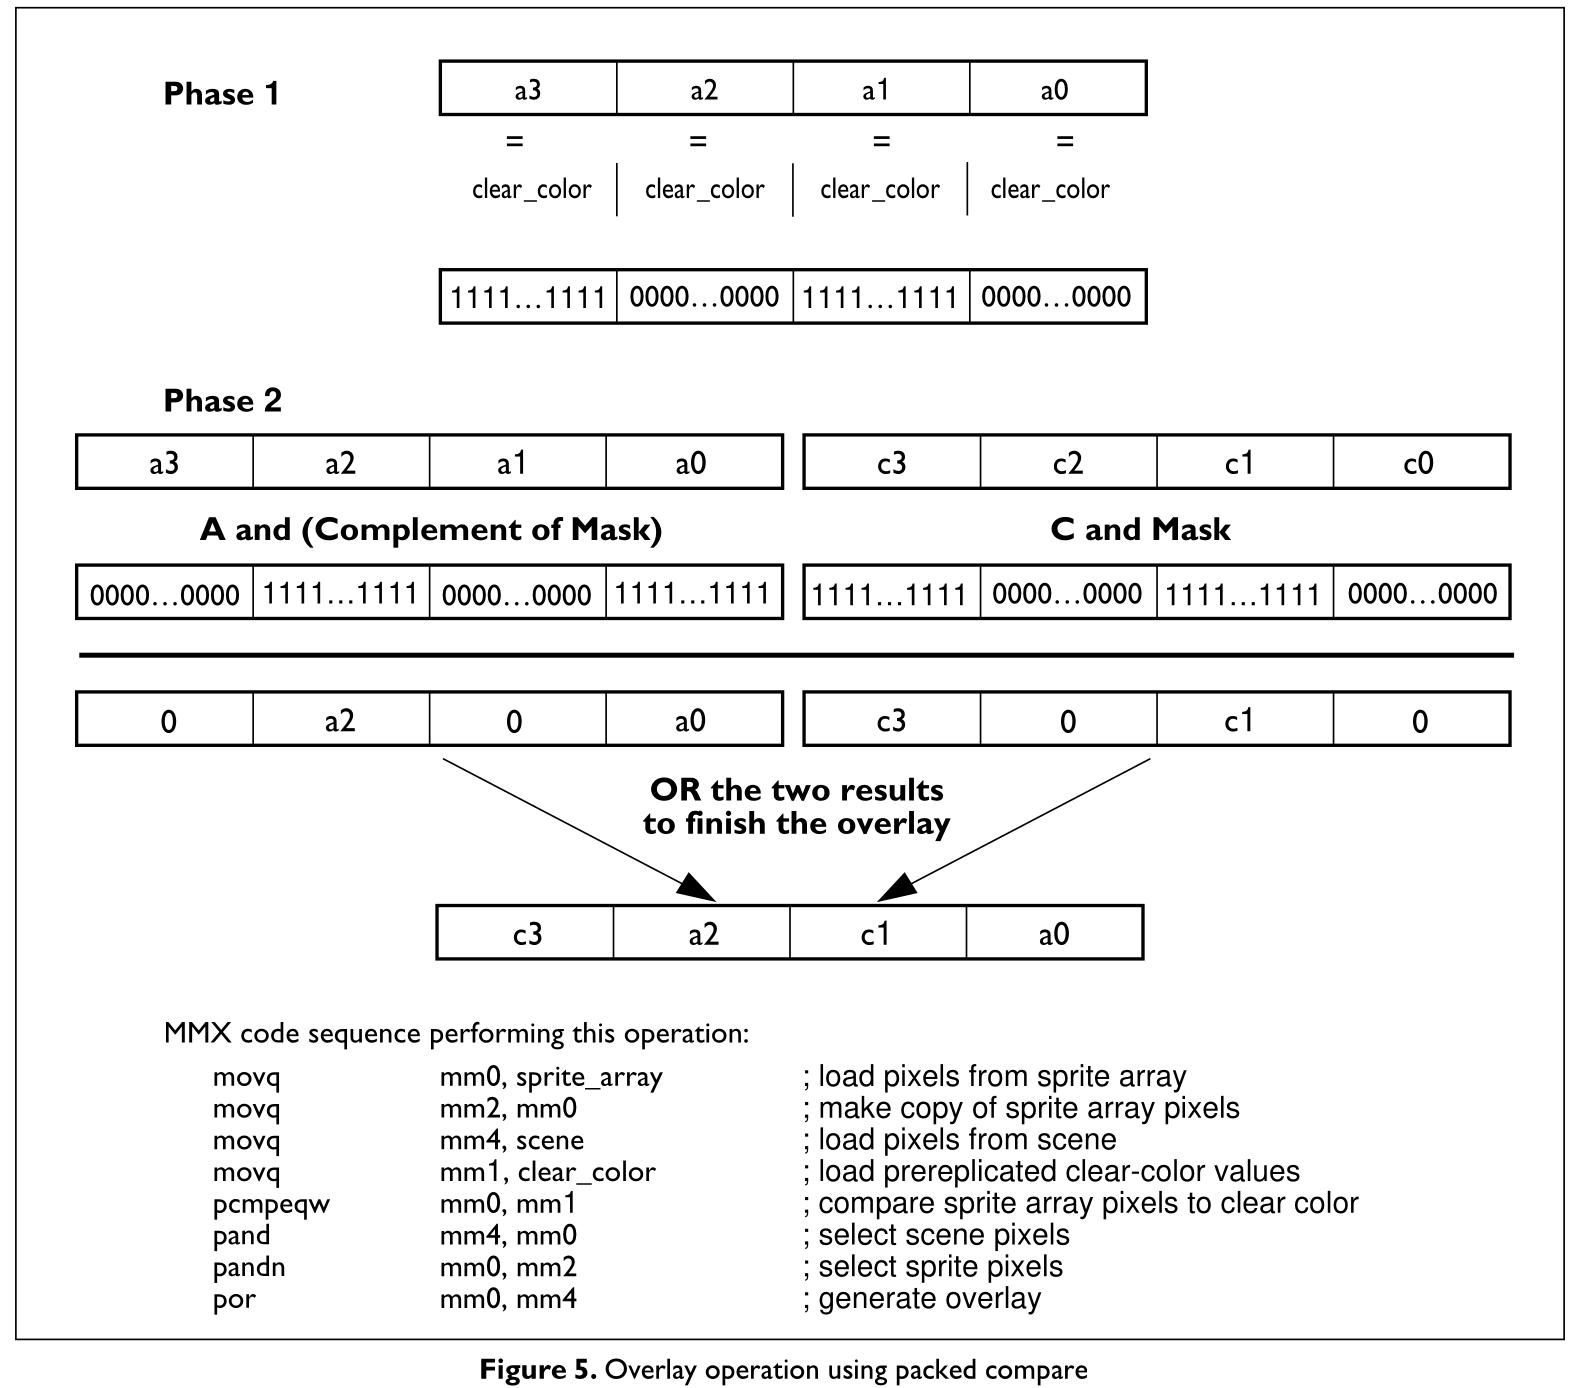
\includegraphics[width=\textwidth]{chapters/07/vectorizing_branches.png}

    ~\\
    In \em Phase 1\em , the mask is computed, i.e. the condition evaluated (the condition is that the color value equals the \texttt{clear\_color} constant).

    Next, in \em Phase 2\em , we evaluate the expressions (in this case it is omitted), and mask the results with the appropriate mask (\texttt{mask}, and $\lnot$\texttt{mask}). Finally, the two results get reduced by a logical or, yielding the final output.

    At the bottom of the graphic is a little assembly code section, emphasizing the fact that the operation can entirely be done with vector instructions.

    \bigskip
    \item[Matrix Transposition] Vector instructions can be fully utilized if the data is stored sequentially in memory. Hence, accessing rows of matrices can vectorized. But I we want to work on the columns of the matrix, it might be beneficial to transpose the matrix. This transposing can be vectorized as well by employing the so called \em unpack \em operation, which interleaves two operands word-wise, as can be seen in the picture:

    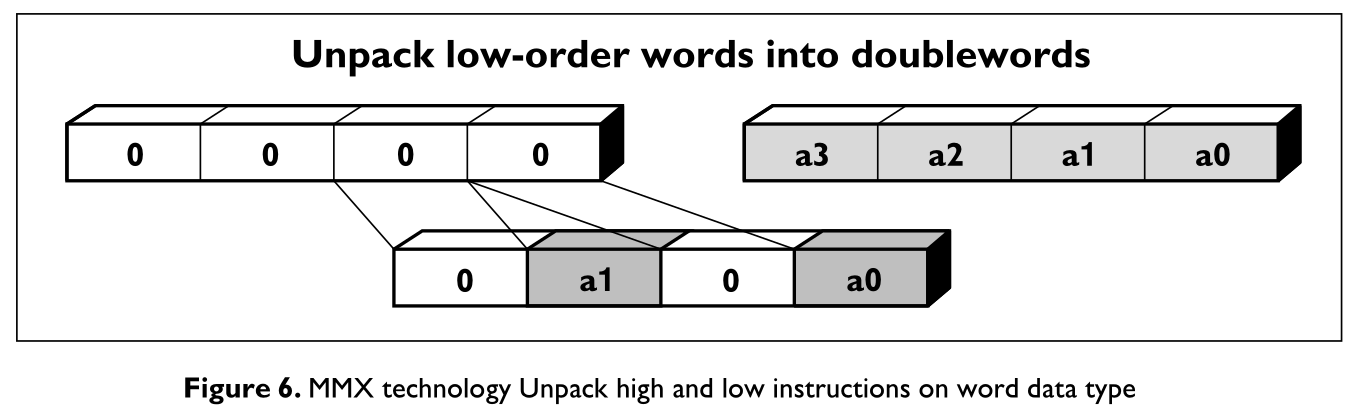
\includegraphics[width=\textwidth]{chapters/07/unpack.png}

    ~\\
    To now transpose an entire matrix we go on like this: Imagine for the sake of simplicity that we have the following matrix $M$:
    \[ M = \begin{pmatrix}
        d3 & d2 & d1 & d0 \\
        c3 & c2 & c1 & c0 \\
        b3 & b2 & b1 & b0 \\
        a3 & a2 & a1 & a0
    \end{pmatrix}\]
    We now compute the last two rows of the matrix by firstly unpacking the last two entries of two adjacent rows, in this case $d$ and $c$, and $b$ and $a$, like shown in \em Phase 1 \em in the following graphic:

    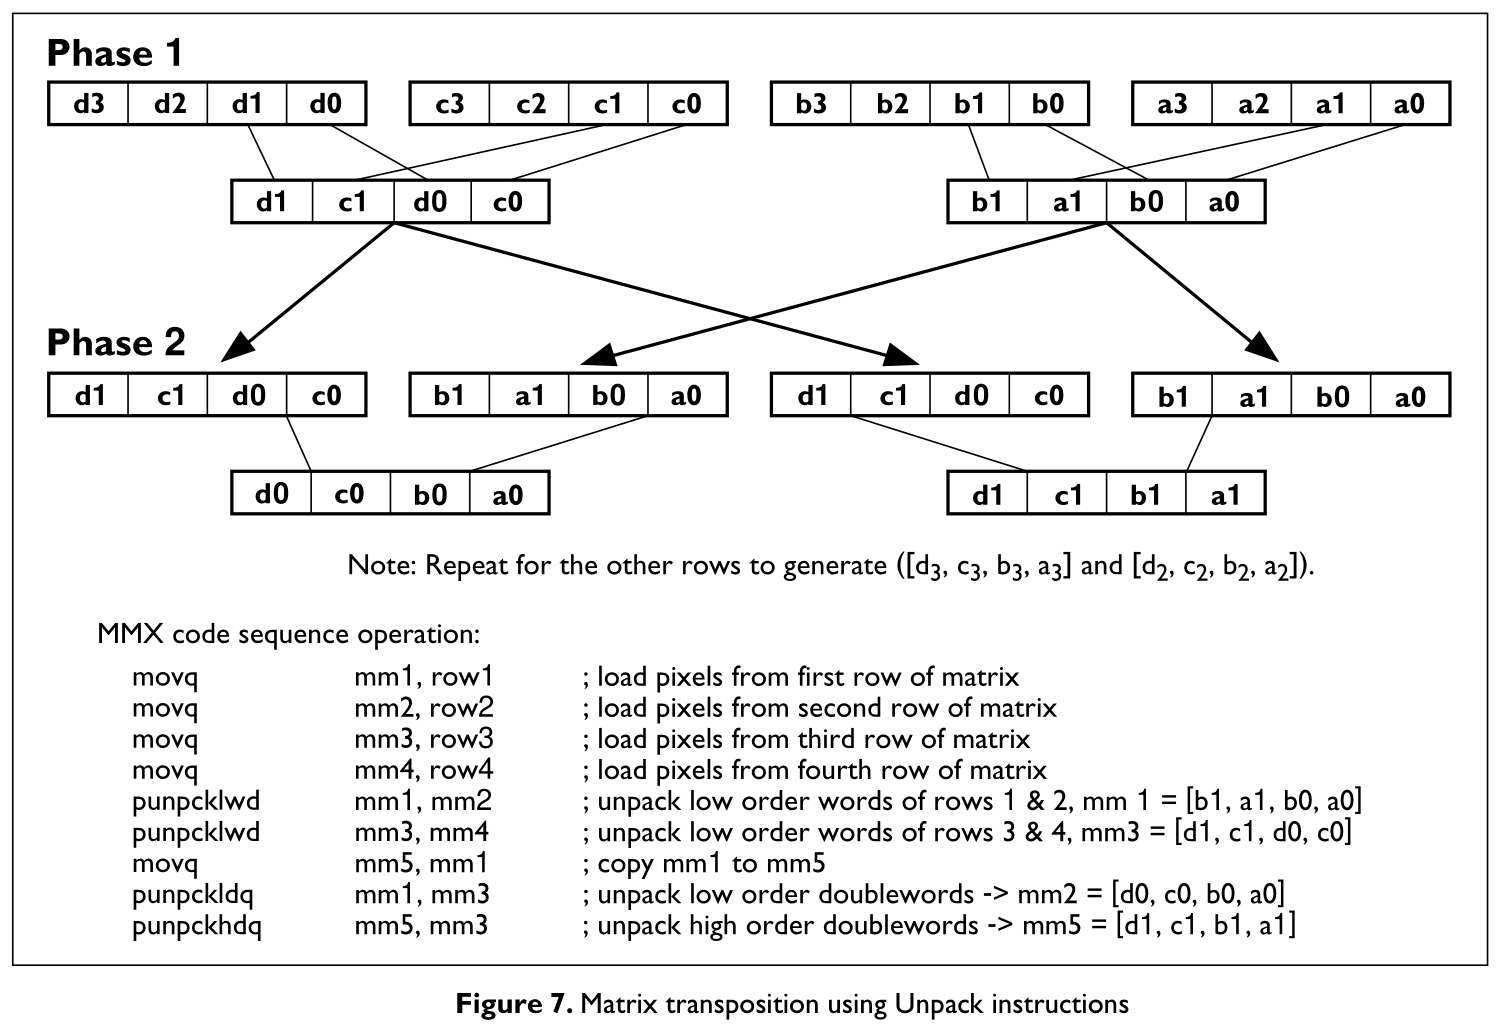
\includegraphics[width=\textwidth]{chapters/07/transpose.png}

    We now created two \em column slices \em of length two in every result of the unpack operations. Thus, we now need to unpack those among themselves, to get longer column slices, or in this case entire columns, as demonstrated in \em Phase 2\em .
    Once again, all the operations can be implemented with vector instructions, as hinted by the small assembly program at the bottom.
\end{description}
\end{document}